\section{Theorie}
\label{sec:Theorie}

\subsection{Grundlagen zur Geometrischen Optik}
\label{subsec:Grundlagen}
In der geometrischen Optik wird Licht als Strahl angenommen. Es zeigt sich, dass
die geometrische Optik für Achsennahe Stahlen eine sehr gute Näherung ist.

Als Grundlegende Versuchsobjekte für die geometrische Optik dienen verschiedene Arten von Linsen, die
auch zu Linsensystemen zusammengefügt werden können. Diese bestehen für gewöhnlich aus einem optisch
dichteren Material, als das umgebende Medium (meistens Luft). Gemäß des Brechungsgesetzes wird
ein auf eine Linse treffender Lichtstrahl beim Eintritt und beim Austritt gebrochen. Die Aufgabe
der geometrischen Optik besteht darin, diese Strahlenverläufe darzustellen und aus ihnen
Aussagen über das erzeugte Bild zu treffen.

Man unterscheidet grundlegend zwischen Sammellinsen und Zerstreuungslinsen. Sammellinsen bündeln
das auf sie einfallende Licht in einem Brennpunkt $F$. Den Abstand zwischen dem Mittelpunkt
der Linse und dem Brennpunkt wird als Brenntweite $f$ bezeichnet. Der Abstand zwischen dem
Mittelpunkt der Linse und dem Gegenstand $G$ wird als Gegenstandsweite $g$, und der Abstand
zwischen dem Mittelpunkt der Linse und dem Ort, an dem das Bild $B$ entsteht, wird als
Bildweite $b$ bezeichnet. Bei Sammellinsen sind Bildweite und Brennweite positiv.
Sammellinsen erzeugen ein reelles Bild. Eine Skizze zu einer dünnen Sammellinse befindet sich in Abbildung
\ref{fig:bikonvex}.

Zerstreuungslinsen hingegen besitzen eine negative Brenn- und Bildweite. Sie erzeugen ein
virtuelles Bild. Eine Skizze zu einer dünnen Zerstreuungslinse befindet sich in Abbildung
\ref{fig:bikonkav}.

\begin{figure}
  \centering
  \begin{subfigure}{0.48\textwidth}
    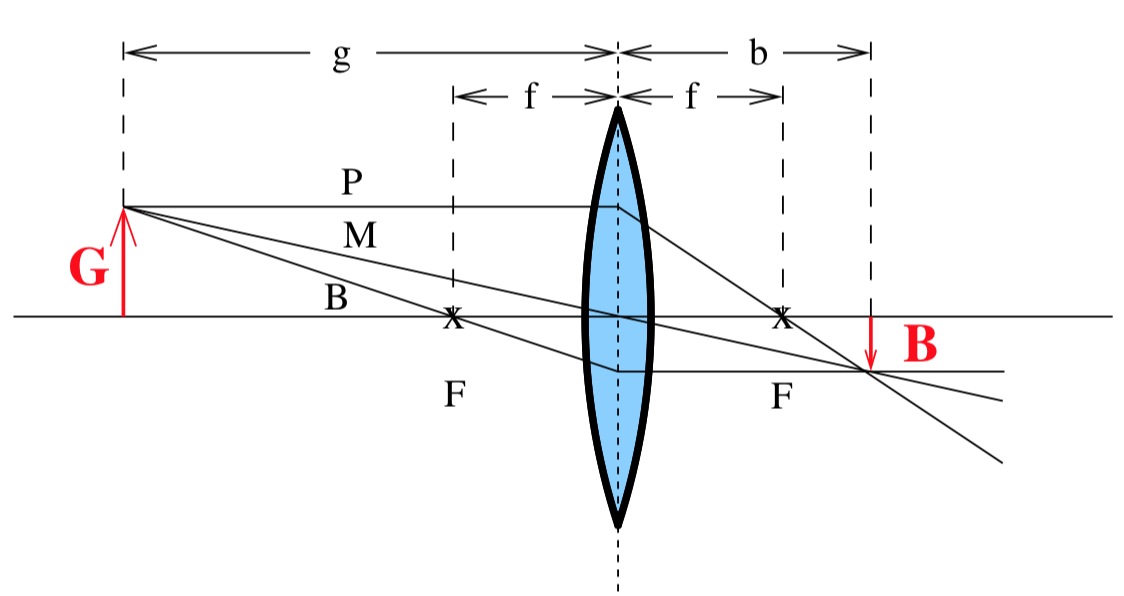
\includegraphics[height=3.5cm]{data/bikonvex.png}
    \caption{Skizze der Funktionsweise einer dünnen Sammellinse \cite{Versuchsanleitung}.}
    \label{fig:bikonvex}
  \end{subfigure}
  \begin{subfigure}{0.48\textwidth}
    \centering
    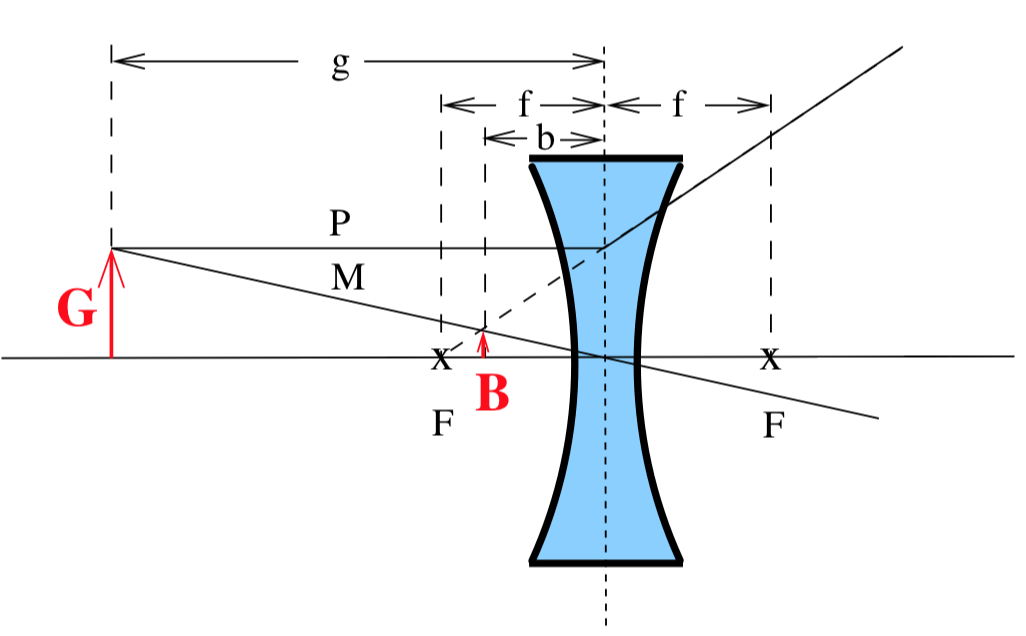
\includegraphics[height=3.5cm]{data/bikonkav.png}
    \caption{Skizze der Funktionsweise einer Zerstreuungslinse \cite{Versuchsanleitung}.}
    \label{fig:bikonkav}
  \end{subfigure}
\end{figure}

Es ist darauf zu achten, dass nur bei dünnen Linsen die Brechung des Lichtes auf die Mittelebene
reduziert werden darf. Bei dicken Linsen müssen zwei Hauptebenen $H$ und $H'$ eingeführt werden,
an denen die Brechung des Lichts vereinfachend angenommen wird. In Abbildung \ref{fig:dick}
befindet sich eine Skizze hierzu.

\begin{figure}
  \centering
  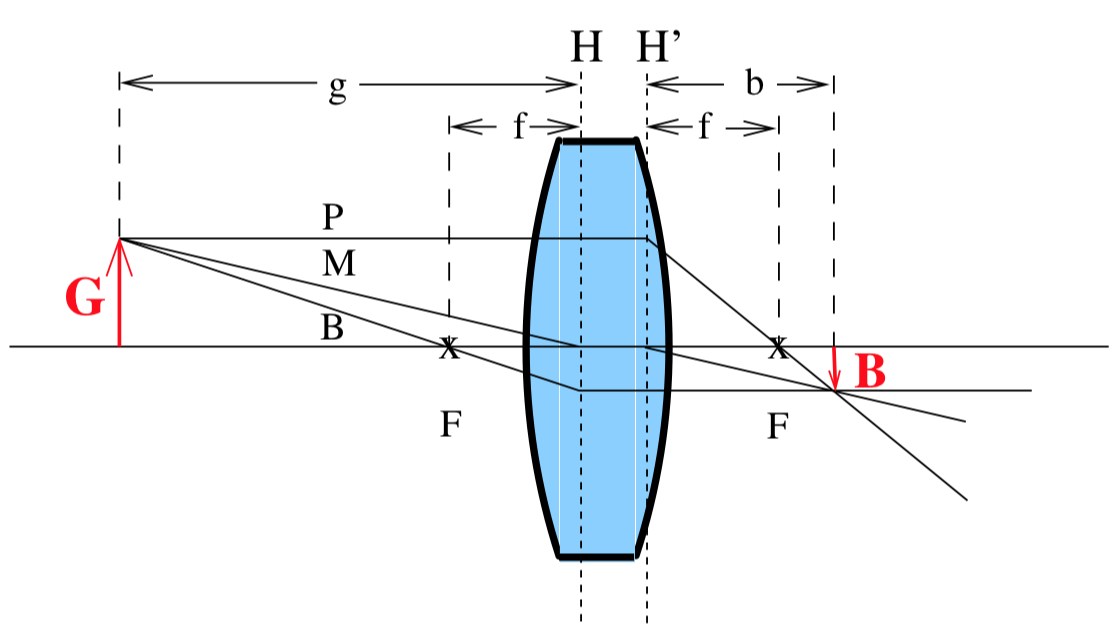
\includegraphics[height=4cm]{data/dick.png}
  \caption{Skizze für den Umgang mit einer dicken Linse \cite{Versuchsanleitung}.}
  \label{fig:dick}
\end{figure}

Zudem muss darauf geachtet werden, dass die Vereinfachung der Brechung an der
Mittelebene bzw. den Hauptebenen nur für achsennah einfallende Strahlen gilt. Achsenfern
einfallende Strahlen werden stärker gebrochen, sodass sich Abbildungsfehler ergeben,
die auch sphärische Abberation genannt werden. Das Bild kann in diesem Fall nicht mehr scharf
dargestellt werden.

Eine weitere Art von Abbildungsfehlern stellt die chromatische Abberation dar. Diese
tritt auf, da kurzwelliges licht stärker gebrochen wird, als langwelliges Licht.

Allgemein sind für die geometrische Bildkonstruktion drei Strahlen von Bedeutung:
Der Parallelstrahl $P$, der vor der Linse parallel zur optischen Achse verläuft und an
der Hauptebene zum Brennpunktstrahl gebrochen wird, der Mittelpunktstrahl $M$, der
durch die Mitte der Linse verläuft und seine Richtung beibehält, und der Brennpunktsrahl
$B$, der vor der Linse durch den Brennpunkt geht und daraufhin an der Hauptebene zum Parallelstrahl
gebrochen wird. Dort, wo alle drei Strahlen sich schneiden, entsteht ein scharfes Bild.

Mithilfe dieser Beziehungen kann unter Verwendung der Stahlensätze das Abbildungsgesetz
\begin{equation}
  V=\frac{B}{G}=\frac{b}{g}
  \label{eqn:V}
\end{equation}
hergeleitet werden. Dabei bezeichnet $B$ die Bildgröße, $G$ die Gegenstandsgröße,
$b$ und $g$ die jeweils entsprechende Weiten und $V$ den Abbildungsmaßstab.
Für dünne Linsen lässt sich zudem die Linsengleichung
\begin{equation}
  \frac{1}{f}=\frac{1}{b}+\frac{1}{g}
  \label{eqn:linsengleichung}
\end{equation}
aufstellen.


\subsection{Verschiedene Methoden zur Bestimmung der Brennweite}
\label{subsec:Methoden}

Zur Bestimmung der Brennweite $f$ einer Linse oder eines Linsensystems gibt es im
Wesentlichen drei verschiedene Methoden.

Eine mögliche Methode ist die Bestimmung der Brennweite durch Messung der Gegenstandsweite
und Bildweite.
Eine weitere Möglichkeit ist die Methode von Bessel. Eine Skizze hierzu befindet sich in
Abbilung \ref{fig:bessel}. Hierbei wird der Abstand zwischen
Gegenstand und Bild konstant gehalten und die Position der Linse variiert, bis zwei
verschiedene Positionen gefunden sind, an denen das Bild scharf ist. Hierbei gelten die
Beziehungen
\begin{align}
  b_1=g_2 \quad \text{und} \quad b_2=g_1\,.\ \\
  \label{eqn:d}
\end{align}
Für $g>b$ ist das Bild verkleinert und für $g<b$ ist das Bild vergrößert. Mithilfe der
Abstände $e=g_1+b_1=g_2+b_2$ und $d=g_1-b_1=g_2-b_2$ lässt sich eine Gleichung für die
Brennweite aufstellen:
\begin{equation}
  f=\frac{e^2-d^2}{4e}
  \label{eqn:bessel}
\end{equation}

Die letzte für diesen Verusch relevante Methode zur Bestimmung der Brennweite ist
die Methode von Abbe. Eine Skizze hierzu befindet sich in Abbilung \ref{fig:abbe}.
Hierbei wird die Brennweite eines Linsensystems über den Abbildungsmaßstab $V$ bestimmt.
Die Bildweite $b$ und die Gegenstandsweite $g$ werden bei einem Linsensystem relativ zu den
Hauptebenen gemessen. Da diese jedoch nicht bekannt sind, wird ein Punkt A gewählt, zu dem
die Bildweite $b'$ und die Gegenstandsweite $g'$ einfach gemessen werden können. Es
gelten dann die folgenden Zusammenhänge:
\begin{align}
  g'=g+h=f\biggl(1+\frac{1}{V}\biggr)+h \,,\\
  b'=b+h'=f(1+V)+h'\,.
\end{align}
Hieraus lässt sich die Brennweite berechnen.

\begin{figure}
  \centering
  \begin{subfigure}{0.48\textwidth}
    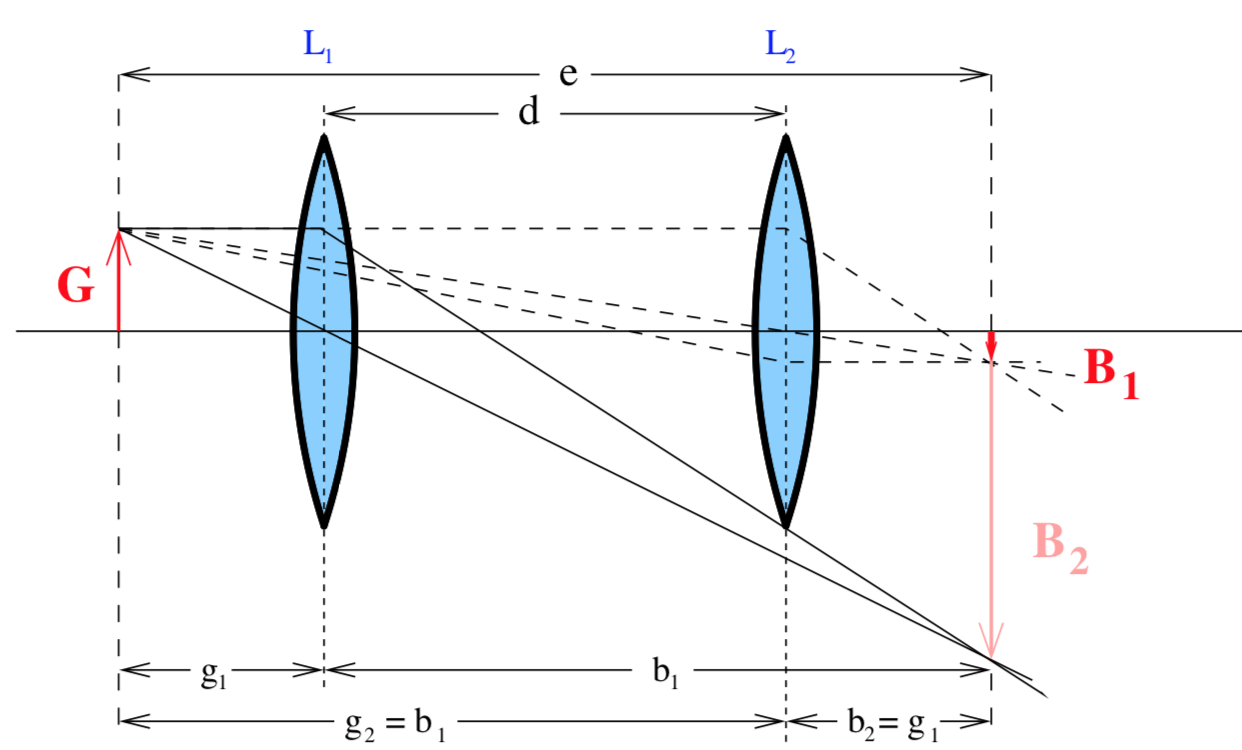
\includegraphics[height=4.1cm]{data/bessel.png}
    \caption{Skizze der Mehtode von Bessel \cite{Versuchsanleitung}.}
    \label{fig:bessel}
  \end{subfigure}
  \begin{subfigure}{0.48\textwidth}
    \centering
    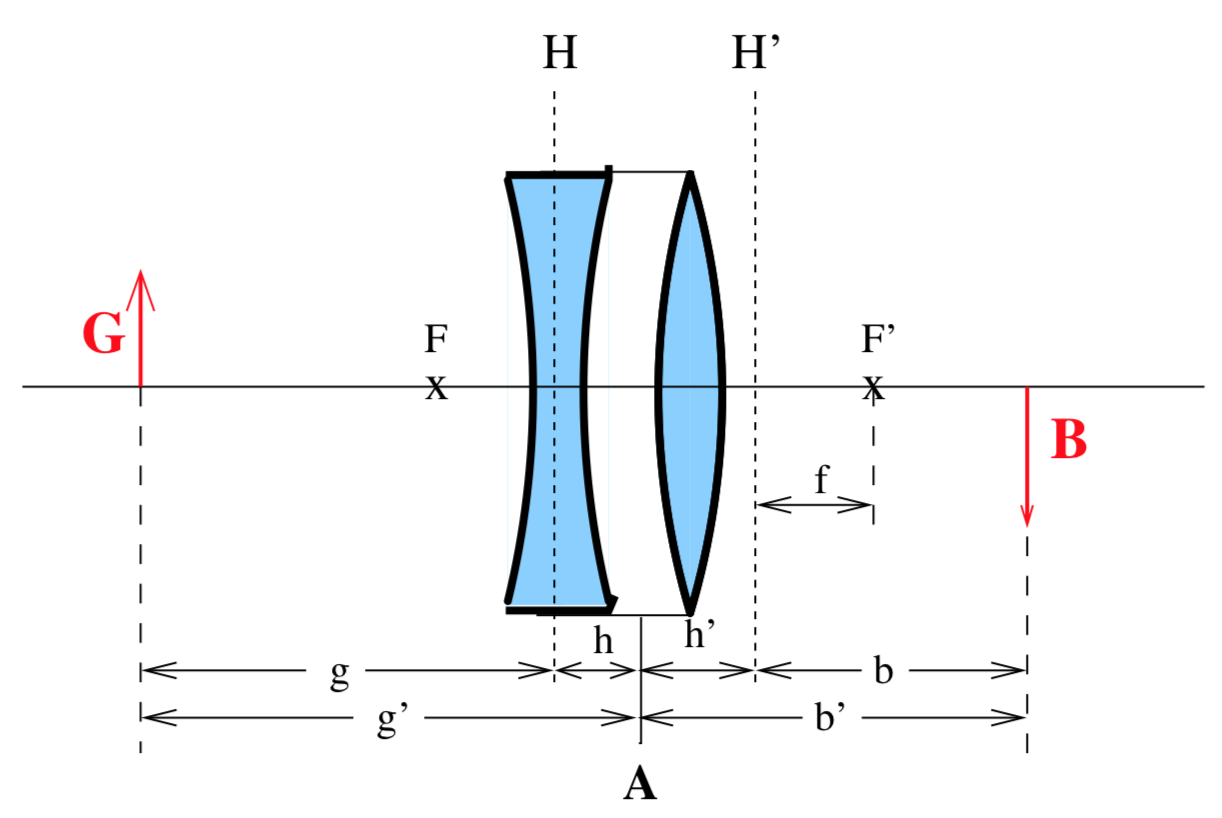
\includegraphics[height=4.1cm]{data/abbe.png}
    \caption{Skizze der Methode von Abbe \cite{Versuchsanleitung}.}
    \label{fig:abbe}
  \end{subfigure}
\end{figure}

Allgemein gilt für ein Linsensystem mit zwei Linsen, die in einem Abstand $d$
voneinander stehen, der Zusammenhang
\begin{equation}
  \frac{1}{f_{\symup{sys}}}=\frac{1}{f_1}+\frac{1}{f_2}-\frac{d}{f_1 f_2} \,.
  \label{eqn:system}
\end{equation}
